\section{Proposed model} \label{sec:model}

Image segmentation models play a vital role in the project and determine the beauty app's latency and user experience. In this section, the proposed CNN is explained, its architecture is about to discuss in more depth. As mentioned previously, as a subset of machine learning, Deep Learning has been showing its accuracy practically in many tasks, such as object detection, object tracking, and object classification. Image segmentation models output a pixel-wise mask of the input image, which is considered as an object segment in the image. Although many DNNs are successful in the image segmentation task in the literature, such as DeepLabV3+ \cite{deeplabv3plus}, PSPNet \cite{pspnet}, they fail to acquire a low latency inference due to their complex architecture in aim to acquire the best accuracy. Considering the requirements, after surveying, I choose U-Net \cite{unet} architecture with MobileNetv2 \cite{mobilenetv2} as a base network for the segmentation tasks. In the following, we dive into the proposed CNN and adaptations to work.
 
 \subsection{MobileNetv2 blackbone}
 MobileNet1 and MobiNetv2 are the first and the second versions in a group of small, low-latency, low-power DNNs named MobileNets. MobileNets is a family of lightweight and general models researched by Google. These models are intended to run with low computational power, such as smartphones, embedded, or IoT devices. Since 2018, when the first version was roll out, there are now three versions with significant improvements after each release. \par
 
 \paragraph{MobiNetv1}
 In MobilNetv1, a key convolution operator called Depth-wise Separable Convolution is first introduced; it takes approximately 70\% less in the number of parameters but only a decrease of 2\% in final accuracy when compared to standard convolution. The basic idea is to replace a full convolutional operator with a factorized one that splits convolution into two separate layers. \par
 
 \begin{figure}[H]
     \centering
     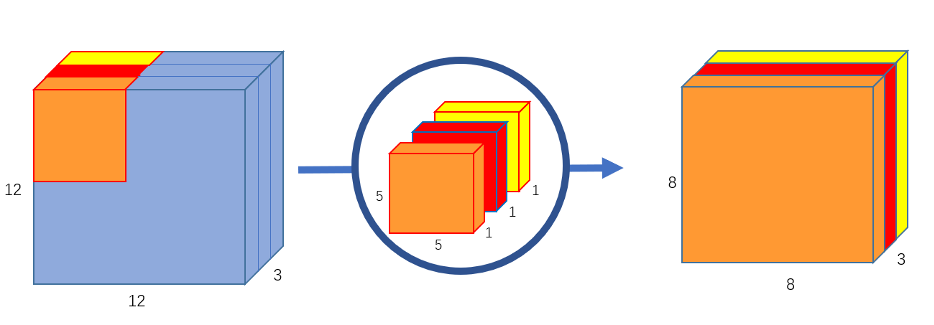
\includegraphics[width=0.9\textwidth]{chapter2/image/mobi1.png}
     \caption{Depthwise convolution, uses 3 kernels (size 5x5) to transform a 12x12x3 image to 8x8x3 image}
     \label{fig:mobi1}
 \end{figure}
 
 \begin{figure}[H]
     \centering
     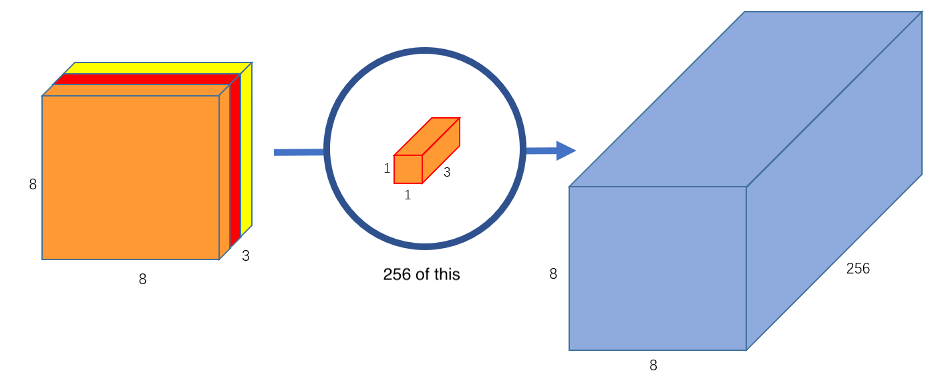
\includegraphics[width=0.9\textwidth]{chapter2/image/mobi2.png}
     \caption{Pointwise convolution, transforms an image of 3 channels (size 8x8x3) to an image of 256 channel (size 8x8x256)}
     \label{fig:mobi2}
 \end{figure}
 
 The entire process can be divvied into two steps: Depthwise convolution and Pointwise convolution. At first, a single-depth convolution is separately applied to each channel of the previous feature map. Take the previous feature map with three channels, illustrated in \textbf{Figure \ref{fig:mobi1}}, Depthwise convolution would consist of three kernels, and each kernel would iterate one channel of the feature map. As the convolutional operations have a single depth, the output has the depth remained the same. Second, N number of Point-wise convolutions are used to combine the outputs of the depth-wise convolution, where N is the desired channel depth of the resulting feature map. In the case of \textbf{Figure \ref{fig:mobi2}}, N is equal to 256. 
 
 \paragraph{MobiNetv2}
 MobileNetV2 is introduced in CVPR 2018, regarded as the next generation of mobile model. It inherits Depthwise Sepratable convolution from MobileNetv1. Although built upon the ideals of MobilNetv1, MobileNetv2 proposes two significant changes to the architecture: linear bottlenecks layers and shortcut connections between the bottlenecks. The basic structure of a bottleneck residual block is shown in \textbf{Figure \ref{fig:mobi2bottleneck}}. \par
 
 \begin{figure}[H]
     \centering
     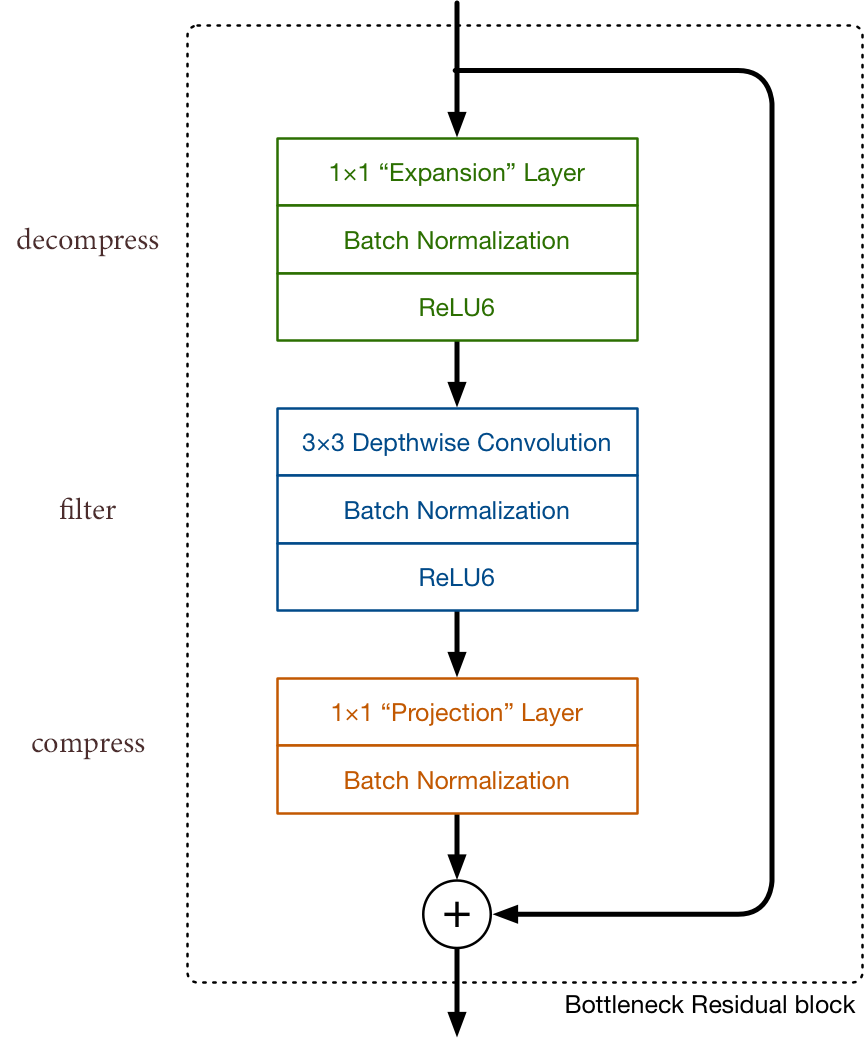
\includegraphics[width=0.6\textwidth]{chapter3/image/block_edited.png}
     \caption{A bottleneck residual block.}
     \label{fig:mobi2bottleneck}
 \end{figure}
There are three convolutional layers in this building block. The first layer is a 1x1 pointwise convolution which is similar to in MobileNetv1.  Its purpose is to expand the number of channels in the data before it goes into the 3x3 depthwise convolution. This expansion layer plays a role as a decompressor that restores the data to its full form. On the other hand, the last convolutional layer, which is also called a bottleneck layer, is a 1x1 pointwise convolution. However, this layer makes the number of channels smaller; in fact, it contrasts to in MobileNetv1 where the pointwise convolution either kept the number of channels the same or doubled them. Its purpose is to projects data with a high number of dimensions (channels) into a tensor with a much lower number of dimensions. In other words, the projection layer compresses the data to make it small again. As a result, the input and the output of the block are low-dimensional tensors, while the filtering step that happens in between is done on a high-dimensional tensor.
 \par
 
 One small change is that the activation function used by MobineNetv2 is ReLU6:
 \begin{equation}
 y = ReLU6(x) = min(max(0, x), 6)
 \end{equation}
 This is like the traditional ReLU as a non-linearity, but it prevents activations from becoming too big. The reason for this is that ReLU6 is more robust than regular ReLU when using low-precision computation. Moreover, the shape of this function is similar to the shape of a sigmoid function. \par
 
 
 I integrate MobinetNetv2 into the overall network excluded the top, which consists of fully-connected layers; otherwise, the image input must be 224x224. MobileNetv2 works as a feature extractor for a second neural network. It is remarked that MobileNetv2 has a good balance between the used resources (memory and FLOPS) and accuracy trade-off. This backbone is far better among other lightweight base networks, such as MnasNet \cite{mnasnet}, SqueezeNet \cite{squeezenet}.
 
 
 \subsection{U-Net architecture} \label{sec:unet}
 This section describes the proposed network entirely. The network is based on the general-purpose U-Net architecture in order to accommodate hair and clothes segmentation tasks. \par
 
 \begin{figure} [H]
     \centering
     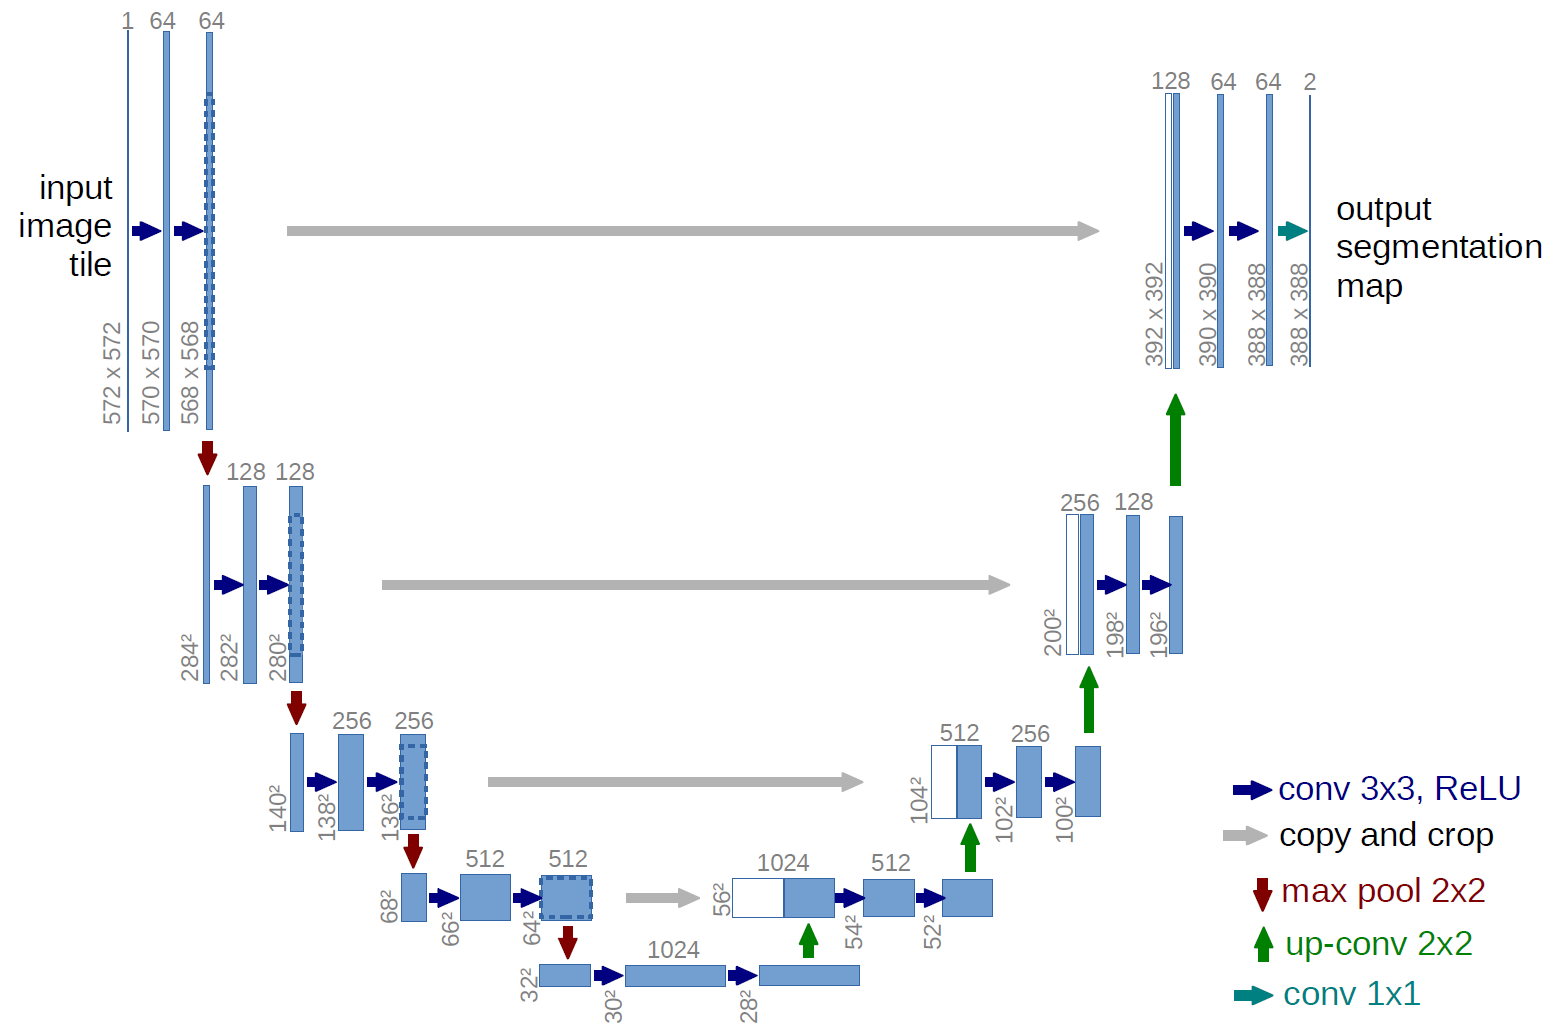
\includegraphics[width=0.7\textwidth]{chapter3/image/u-net.png}
     \caption{Illustration for U-shaped architecture in the origin paper \cite{unet}.}
     \label{fig:unet1}
 \end{figure}
 
 U-Net is an autoencoder type network architecture introduced in \cite{unet} for semantic segmentation of biomedical images in 2015. However, U-Net achieves high accuracy in other segmentation tasks as well. It introduces skip-connections to the autoencoder architecture to improve resolving and propagating higher-level features in the decoder block.
As a consequence, the decoder can access information from the encoder, such as edges, corners and angles in the original images. Many semantic segmentation networks utilize this ideal where information from the encoder is passed to the decoder via long skip-connections to preserve higher-level information found at higher resolutions in the encoder. \par

\vspace{5mm}

 \begin{figure} [H]
     \centering
     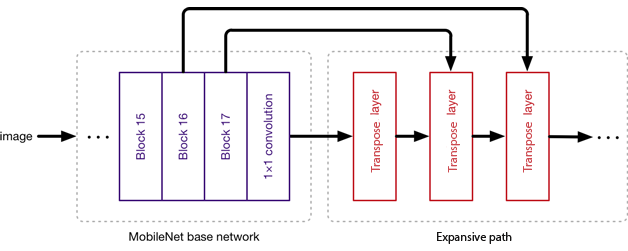
\includegraphics[width=0.9\textwidth]{chapter3/image/architec.png}
     \caption{UNet architecture with the MobileNetv2 base model.}
     \label{fig:unet2}
 \end{figure}
 
 While \textbf{Figure \ref{fig:unet1}} depicts the origin U-Net architecture in view of layers, \textbf{Figure \ref{fig:unet2}} shows the adapted network in view of components. More specifically, the contracting path replicates the architecture of MobileNetv2 with 17 blocks in total. On the other hand, the expansive path consists of an upsampling of feature maps followed by a 2x2 convolution that halves the number of feature channels. The upsampling method is transposed convolutions. The number of max-pooling layers 
 equal to the number of transposed convolutions and equals five. Generally, the proposed network has the same architecture as the original version; however, I made slight modifications.
 The first adaptation I made is that batch normalization is only used in the contracting path of the network. It changes results from preliminary experiments and increases the speed of the network without decreasing the accuracy. The second adaptation lies at the two last layers, where the last convolution has a kernel size of one and is followed by a softmax activation. As a result, the network would output a final probability map, which represents the desired mask. Following that, the loss is calculated as a binary cross-entropy function on a pixel-wise basis.
 \par